%%%%%%%%%%%%%%%%%%%%%%%%%%%%%%%%%%%%%%%%%
% Template LaTeX
% Versão 0.1 (29/10/2018)
%
% Este template foi desenvolvido para o II WPPGEEC
% https://sites.google.com/view/upm-wppgeec/p%C3%A1gina-inicial
%
%%%%%%%%%%%%%%%%%%%%%%%%%%%%%%%%%%%%%%%%%

%---------------------------------------------------------------------------------
%%% Document configuration - Do not change
\documentclass[a4paper,12pt]{article}
\usepackage{geometry}
\geometry{
	a4paper,
	total={180mm,257mm},
	left=15mm,
	top=10mm,
}
\usepackage{fancyhdr}
\usepackage[pdftex]{graphicx} 
\pagestyle{fancy}
\fancyhf{}
\fancyfoot[CE,CO]{II-WPPGEEC Proceedings, São Paulo, SP,  v.2, out. 2019}
\fancyfoot[LE,RO]{\thepage}
\fancypagestyle{plain}{\pagestyle{fancy}}
\usepackage[utf8]{inputenc}
\usepackage{indentfirst}

%\ifCLASSOPTIONcompsoc                        % AAB inserido
\usepackage[caption=false,font=normalsize,labelfont=sf,textfont=sf]{subfig}
%\else
%\usepackage[caption=false,font=footnotesize]{subfig}
%\fi
%%%
%---------------------------------------------------------------------------------

\usepackage[english]{babel} % Pacote para lingua inglesa
%\usepackage[portuges]{babel} % Pcote para lingua portuguesa
\graphicspath{{../../Dissertacao/figuras/}}

\title{Fusion of Evidences for Edge Detection in PolSAR Images }
\author{%
	\textsc{Anderson Adaime de Borba}\\ % Primeiro autor
	\normalsize Universidade Presbiteriana Mackenzie - IBMEC-SP \\ % Instituição primeiro autor
	\and
	\textsc{Mauricio Marengoni}\\% Orientador 
	\normalsize Universidade Presbiteriana Mackenzie \\ % Instituição segundo autor
        \and
	\textsc{Alejandro C. Frery}\\% Coorientador autor
	\normalsize Universidade Federal de Alagoas \\ % Instituição segundo autor
}
\date{\today}

\begin{document}
	\maketitle
	\begin{abstract}
Polarimetric Synthetic Aperture Radar (PolSAR) has achieved an important position as a remote sensing imaging method. 
However, PolSAR images are contaminated with speckle noise, making its processing and analysis challenging tasks. 
The present study discusses a detection method based on the fusion of evidences obtained in the intensity channels of multilook PolSAR images.
The method consists of detecting transition points in the finest strip of data which spans two regions using the maximum likelihood.
This is applied to each of the three intensity channels (hh), (hv) and (vv). 
The fusion methods are simple average, stationary wavelet transform (SWT), principal component analysis (PCA), and ROC statistics.  
The results indicate improvement performance of the approach in detecting edges with possible paths for future research.
		\textbf{Keywords: PolSAR, edge detection, maximum likelihood estimation, fusion.} 
	\end{abstract}
	
	\section{INTRODUCTION} \label{sec:introduction}
		  This work presents results on the detection and fusion of edge evidence applied to Polarimetric Synthetic Aperture Radar images (PolSAR). Models and algorithms as required for appropriate treatment of their special statistical characteristics were employed.

Among the available edge detection techniques for SAR imagery, it is worth mentioning those based on the gradient, Refs.~\cite{tlb, obw, flmc, fyf}, and on Markov chains, Ref.~\cite{bf}. The former suffers from the effect of speckle, and the latter leads to computer-intensive methods. Ref.~\cite{gfn} presents a comparison between several edge detectors. 

Alternatively, techniques based on statistical modeling have been used in edge detection, Refs.~\cite{gmbf, fbgm, horrit, gfn} and, more recently,  utilizing \textit{Deep Learning}, Refs.~\cite{bac, ztmxzxf, tabmm, xstz}.

This work relies on ideas stemming from information fusion.
This approach has been followed by Refs.~\cite{sglmla,sg} in order to extract valuable knowledge from remotely sensed data.

This work follows the statistical modeling approach, mainly the techniques described in Refs.~\cite{fbgm, nhfc} using the Wishart distribution.
The basis for the fusion of information is described in Refs.~\cite{mit, sg}. 


The objective of this work shows the viability of a procedure for edge detection in each channel of a PolSAR image and then performed the fusion of evidences. The intent is understanding and quantifying the importance of the information provided by each channel in order to better edge detection.

	\section{METHODS} \label{sec:method}
Most of the usual techniques for edge detection, e.g., 
Sobel, Canny, Laplacian of Gaussian (LoG) and pyramidal LoG, assume additive Gaussian noise and, thus, they are ineffective for PolSAR imagery.
The noise in these kinds of images is multiplicative, making edge detection in SAR images a challenging task.

The main idea for edge detection is based on Ref.~\cite{nhfc, gmbf} and show how to detect the transition point in a thin strip between two regions of the image. The transition point is considered as edge evidence. 

The following procedure is proposed:
\begin{enumerate}
	\item identify the centroid of a region of interest (ROI) in an automatic, semi-automatic or manual manner;
	\item cast rays from the centroid to the outside of the area;
	\item collect data around the rays using the  Bresenham's midpoint line algorithm, ideally the size of a pixel;
	\item detect points in the data strips which provide evidence of changes in their statistical properties, i.e., a transition point that defines edge evidence;
	\item use the Generalized Simulated Annealing (GenSA) method, Ref.~\cite{xgsh}, to find maximum points in the functions of interest;
	\item fuse the evidence of detected edges in the $(hh)$, $(hv)$ and $(vv)$ channels using simple average, PCA, SWT and ROC curve.
\end{enumerate}
With this, fully polarized data is not required, only the intensity channels.
	\section{PARTIALS RESULTS} \label{sec:part_result}
The PolSAR image of the Flevoland region in the Netherlands is used, with $4$ looks, for the numerical tests. 
Fig.~(\ref{flevoland_radial_4look}) shows the region of interest, with the radial lines for edge detection.

\begin{figure}[hbt]
\centering
	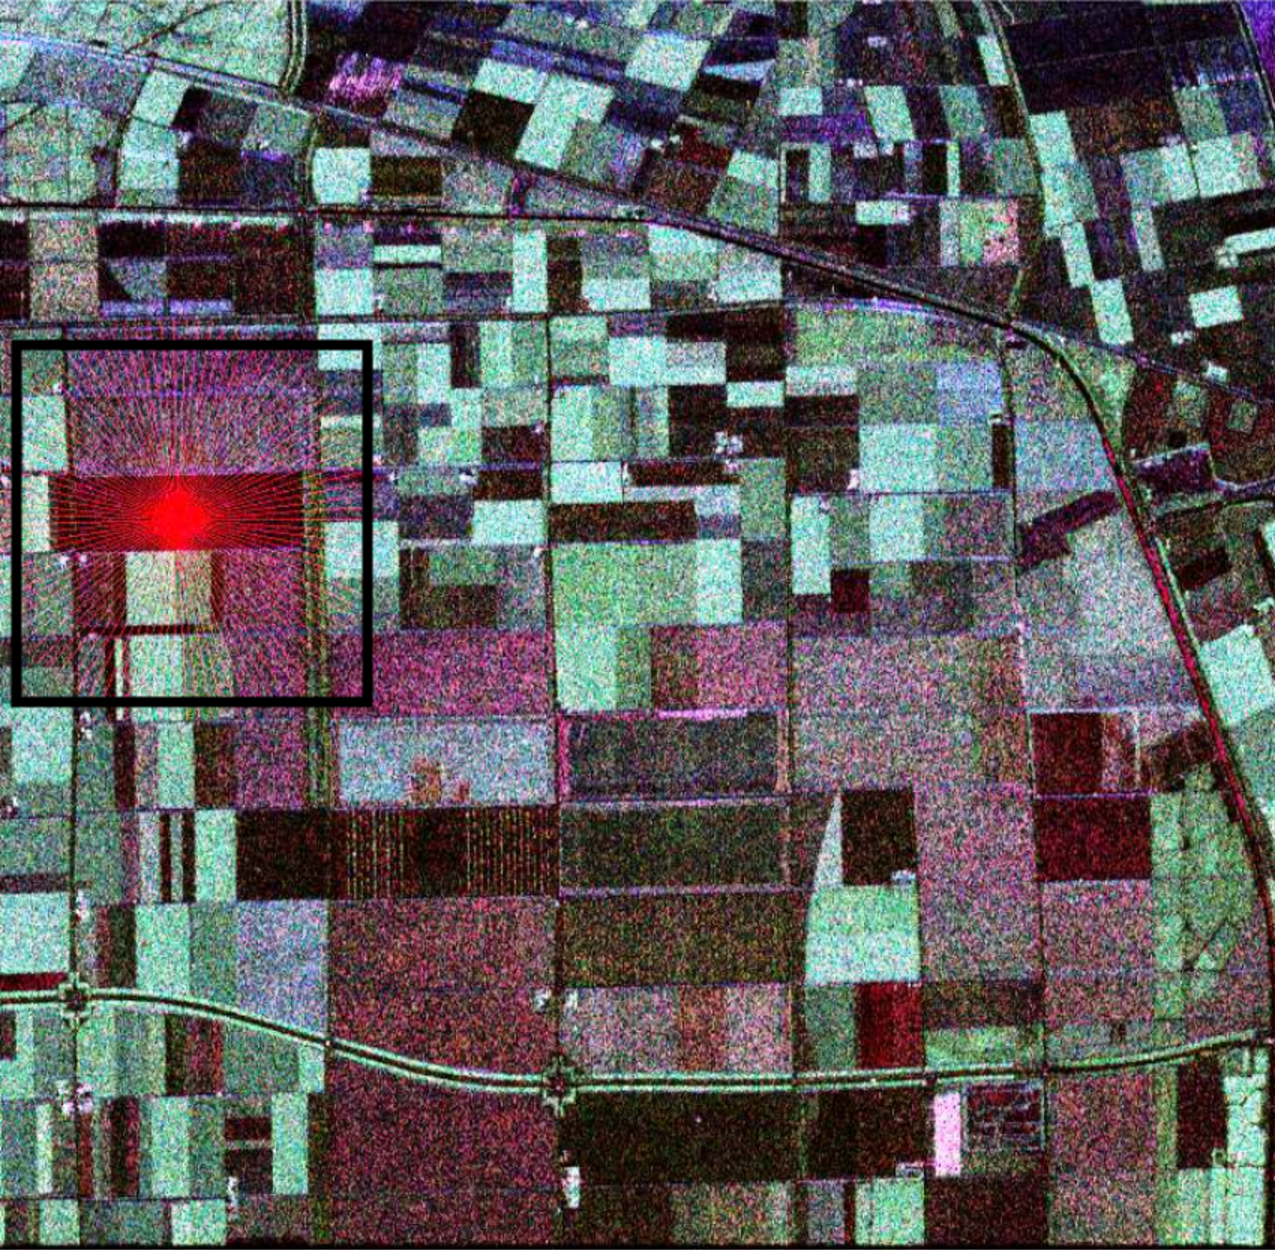
\includegraphics[width=\linewidth]{flevoland_radial_4_look_black}
	\caption{Region of interest (ROI) in the image of Flevoland.}
\label{flevoland_radial_4look}
\end{figure}

Figs.~\ref{evidencias_hh_hv_vv}\subref{evidencias_hh_hv_vv:a}, \subref{evidencias_hh_hv_vv:b} and~\subref{evidencias_hh_hv_vv:c} show, respectively, the edge evidence in the $hh$, $hv$ and $vv$ channels. 
The algorithm achieves better accuracy in channels $hh$ and $hv$ than in channel $vv$.  

It is noteworthy that GenSA identified the maximum evidence correctly, even in the presence of multiple local maxima as in the case of the $vv$ channel.

\begin{figure*}[hbt]
	\centering
     \subfloat[Evidences in channel $hh$ \label{evidencias_hh_hv_vv:a}]{%
       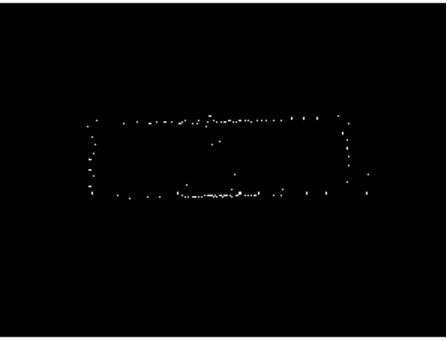
\includegraphics[width=0.32\linewidth]{flevoland_hh_evid_crop_teste}
     }
     \subfloat[Evidences in channel $hv$ \label{evidencias_hh_hv_vv:b}]{%
       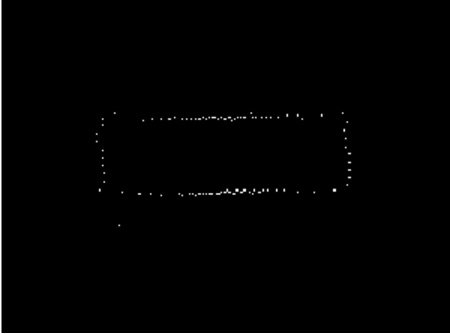
\includegraphics[width=0.32\linewidth]{flevoland_hv_evid_crop_teste}
     }
     \subfloat[Evidences in channel $vv$ \label{evidencias_hh_hv_vv:c}]{%
       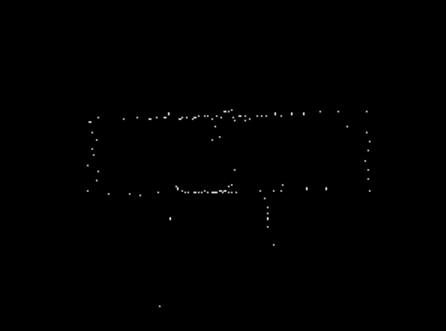
\includegraphics[width=0.32\linewidth]{flevoland_vv_evid_crop_teste}
     }
     \caption{Edges evidences}
     \label{evidencias_hh_hv_vv}
   \end{figure*}

Figs.~\ref{fusion_met}\subref{fusion_met:a}, \subref{fusion_met:b}, \subref{fusion_met:c}, and~\subref{fusion_met:d} show, respectively, the results of fusing these evidences. The methods use all the pixels detected in the three channels by using different weights: 
the average weights the pixels equally, SWT finds the coefficients of the linear combination of its wavelet bases, and PCA weights by the eigenvalues of the covariance matrix.

The ROC statistics method does not use all pixels of the channels, because the method is based on thresholds for discarding pixels. 
This was observed in Fig.~\ref{fusion_met}\subref{fusion_met:d}.

\begin{figure*}[hbt]
	\centering
     \subfloat[Average fusion\label{fusion_met:a}]{%
       %\includegraphics[width=0.2\textwidth]{example-image-a}
       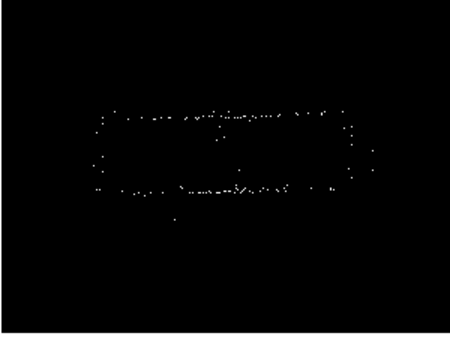
\includegraphics[width=0.32\linewidth]{flevoland_fusao_media_crop_teste}
     }
     \subfloat[SWT fusion\label{fusion_met:b}]{%
       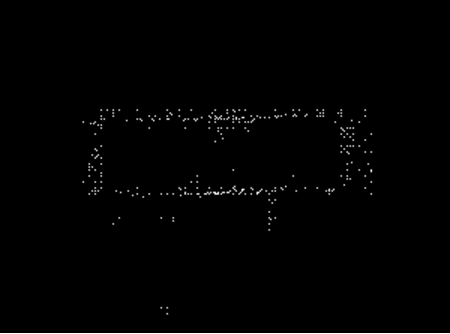
\includegraphics[width=0.32\linewidth]{flevoland_fusao_swt_crop_teste}
     }
     \subfloat[PCA fusion \label{fusion_met:c}]{%
       %\includegraphics[width=0.2\textwidth]{example-image-a}
       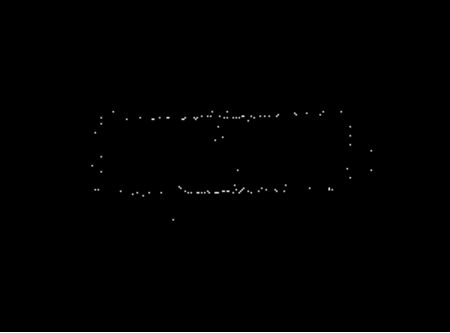
\includegraphics[width=0.32\linewidth]{flevoland_fusao_pca_crop_teste}       
     }\\
     \subfloat[ROC fusion\label{fusion_met:d}]{%
       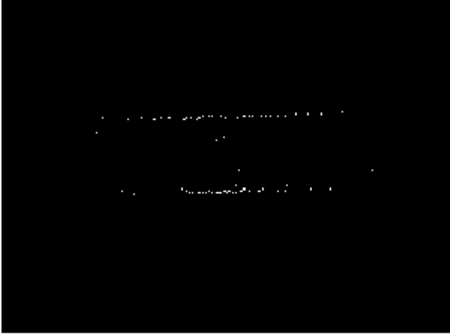
\includegraphics[width=0.32\linewidth]{flevoland_fusao_roc_crop_teste.pdf}
     }
     \caption{Fusion methods}
     \label{fusion_met}
\end{figure*}



	\section{CONCLUSION}
In this article, methods for fusion of edges evidence in PolSAR images. 
First, edges evidence were found using the method of maximum likelihood in the three intensities channels. 
Second, fusion methods were applied, simple average, SWT, PCA, and ROC curve. A simulated image was used to quantify and compare the results. 

The detection was performed by maximum likelihood, in which the function is not smooth and presents many local maximal.
Therefore, the difficulty of using classical optimization methods was stressed. 
To solve this problem, Simulated Annealing was applied because it is appropriate to optimize non-differentiable functions.

The quality of the fusion with the probability of detecting the edge was correctly measured. There is an improvement in detecting evidence of edges in the intensity channels.

From the obtained results, the viability of increasing the number of channels used for edge evidence detection was identified, paving the way to research new fusion methods in PolSAR image.

	\bibliographystyle{IEEEtran}
	\bibliography{../../../Text/bibliografia}
\end{document}
